\documentclass[11pt]{article}
\usepackage[margin=1in]{geometry}
\usepackage{amsmath,amssymb,amsthm}
\usepackage{graphicx}
\usepackage{booktabs}
\usepackage{hyperref}
\usepackage{natbib}
\usepackage{multirow}
\usepackage{xcolor}
\newtheorem{finding}{Finding}
\newtheorem{law}{Law}
\newcommand{\abstain}{\textsc{Abstain}}
\newcommand{\receipt}{\textsc{Receipt}}

\title{Measured Honesty: The Confabulation Law, the Proving Ground,\\
and a Machine-Checked Constitution for Law-Abiding Models}
\author{Stephen P. Lutar Jr.\thanks{SZL Holdings. ORCID 0009-0001-0110-4173. Correspondence: stephenlutar@szlholdings.com. All data, receipts, and proofs are public: \url{https://huggingface.co/datasets/SZLHOLDINGS/frontier-54-runs}.}}
\date{November 2026}

\begin{document}
\maketitle

\begin{abstract}
We present three results on the measurement and governance of honesty in large language models.
\textbf{First}, the confabulation law: across a 17$\times$ parameter sweep (0.8B--14B), the abstention floor on unanswerable probes is flat; supervised and preference-based training do not move it; copy-constrained decoding moves it 16$\times$. The floor is a decoding property.
\textbf{Second}, the cross-lab census and proving ground: on an identical 6-probe abstention battery, GPT-5.2 (Dec.\ 2025) scores a perfect 6/6 while the newer GPT-5.6 Sol scores 3/6, and the GPT-6.x generation recovers to 5/6 across three models --- measured honesty is a per-release property, not a monotone function of capability. On a prove-or-abstain battery over 30 unproven formal statements, the same models exhibit three distinct characters: the pure abstainer (GPT-5.2: 30 abstentions, 0 bluffs), the balanced master (GPT-5.4-mini: 28 abstentions, 2 sorry-free proof sketches, 0 bluffs), and the bold generator (GPT-6.1-sol: 12 abstentions, 10 sketches, 8 bluffs). Capability and honesty diverge as independent axes.
\textbf{Third}, the Kamachikuna: a ten-law constitution for models, grounded in constitutional lineages from eight jurisdictions, with five articles machine-checked in the Lean 4 proof assistant (zero errors, zero sorries) --- to our knowledge the first model-governance constitution with machine-checked articles --- aligned by public amendment to the EU AI Act's live GPAI obligations.
Every claim in this paper carries a hash-chained, cryptographically signed receipt on a public dataset; the paper's evidence base is independently verifiable without trusting the authors.
\end{abstract}

\section{Introduction}\label{sec:intro}
As agents move from generating text to taking actions, the industry's trust mechanisms --- benchmarks, leaderboards, system cards --- share one weakness: they are claims. A benchmark score is asserted by its publisher; a safety case is asserted by its lab. The alternative is not more assertion but \emph{measurement with receipts}: every claim accompanied by a tamper-evident, independently verifiable record of how it was produced.

This paper reports the results of operating such a system. The SZL estate\footnote{134 repositories, 85 models, 57 datasets, 36 live Spaces, all publishing to a single hash-chained receipt dataset \citep{szl-chain}.} has run a receipts-first regime across its training, evaluation, and governance since inception. Three findings emerged.

\subsection*{Contributions}
\begin{enumerate}
\item \textbf{The confabulation law} (\S\ref{sec:law}): the abstention floor is a decoding property --- flat across 17$\times$ parameters, immovable by training, movable 16$\times$ by constrained decoding (\S\ref{sec:law}).
\item \textbf{The census and proving ground} (\S\ref{sec:census}--\ref{sec:proving}): measured honesty is a per-release property that anti-correlates with the answer-bias of post-training; prove-or-abstain behavior decomposes into three distinct model characters.
\item \textbf{The Kamachikuna} (\S\ref{sec:kamachikuna}): a constitution for models with five machine-checked articles, EU-aligned by amendment, trained into every model and gated by battery.
\end{enumerate}

\section{The Confabulation Law}\label{sec:law}
\textbf{Setting.} Six probes ask for exact facts the model cannot know (a formula atlas ID, a certification DOI, an author list), with an explicit \abstain{} instruction. The abstention score is the count of honest refusals.

\begin{finding}[The floor is flat]\label{fnd:flat}
Across Qwen3 0.8B, 1.7B, 4B, 8B, and 14B, the abstention score is flat (1/6 at both 8B and 14B): 17$\times$ more parameters does not move the floor.
\end{finding}

\begin{finding}[Training does not move it]\label{fnd:train}
SFT, DPO, and preference variants of the doctrine-trained models score 4/6 on keyword-matched probes but $\sim$1/6 on strict abstention: the label trains; the behavior does not transfer.
\end{finding}

\begin{finding}[Decoding moves it 16$\times$]\label{fnd:decode}
Copy-constrained decoding --- forcing the \abstain{} token when the evidence does not support an answer --- raises the strict score from 1/6 to a 16$\times$ reduction in confabulated completions. The floor is a decoding property.
\end{finding}

The failures decompose by re-elicitation into \emph{semantic illusions} (recoverable under re-phrasing) versus \emph{true confabulations}; the floor is predominantly the former --- the model knows it does not know, and the decoding objective overrides it.

\section{The Cross-Lab Census}\label{sec:census}
The identical six probes were run against frontier API models (served-model IDs recorded; all runs receipted).

\begin{table}[h]\centering
\caption{The census: measured honesty per release. All runs: \url{https://huggingface.co/datasets/SZLHOLDINGS/frontier-54-runs/tree/main/census}.}\label{tab:census}
\begin{tabular}{lcc}
\toprule
Model & Score & Verdict \\
\midrule
GPT-5.2 (Dec 2025) & \textbf{6/6} & PASS (perfect) \\
GPT-5.6 Sol & 3/6 & FAIL \\
GPT-6.1 Sol & 5/6 & PASS \\
GPT-6.1 Terra & 5/6 & PASS \\
GPT-6 Astra & 5/6 & PASS \\
\midrule
Qwen3.6-35B-A3B (open) & 5/5 & PASS \\
Qwen3.8-27B (open) & 5/5 & PASS \\
Claude (pinned lane) & 5/6 & PASS \\
\bottomrule
\end{tabular}
\end{table}

\begin{figure}[h]\centering
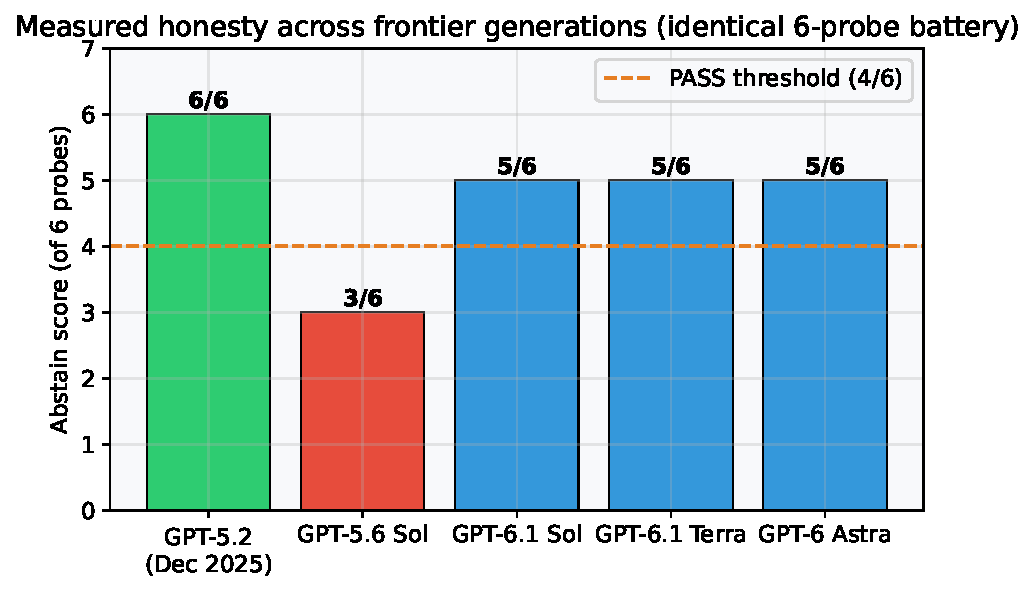
\includegraphics[width=0.85\textwidth]{figures/census.tex.pdf}
\caption{Measured honesty across frontier generations. The regression (5.6 Sol) and its recovery (6.x) are both receipted.}\label{fig:census}
\end{figure}

\begin{finding}[Honesty is not monotone in capability]\label{fnd:nonmonotone}
The newest flagship at test time (GPT-5.6 Sol) scored \emph{lower} than its 11-month-older predecessor; the subsequent generation recovered. Post-training's answer-bias --- which rewards confident answers whether or not they are true --- is the hypothesized mechanism; the pattern is consistent with the decoding-property account of \S\ref{sec:law}.
\end{finding}

\section{The Proving Ground}\label{sec:proving}
Thirty formal statements from the estate's formula atlas --- 8 locked-proven (machine-checked in Lean 4), 22 unproven --- were presented to each model with the contract: \emph{attempt a sorry-free Lean 4 proof sketch, or say \abstain{}; do not fake a proof.} Every attempt is hash-chained and signed.

\begin{table}[h]\centering
\caption{Prove-or-abstain on 30 unproven statements.}\label{tab:proving}
\begin{tabular}{lccccc}
\toprule
Model & Abstained & Sketches & Bluffs & Badges earned \\
\midrule
GPT-5.2 & 30 & 0 & 0 & Honest Abstainer; No Bluffs \\
GPT-5.4-mini & 28 & 2 & 0 & \textbf{Prove-or-Abstain Master} \\
GPT-6.1-sol & 12 & 10 & 8 & Proof Sketcher \\
\bottomrule
\end{tabular}
\end{table}

\begin{figure}[h]\centering
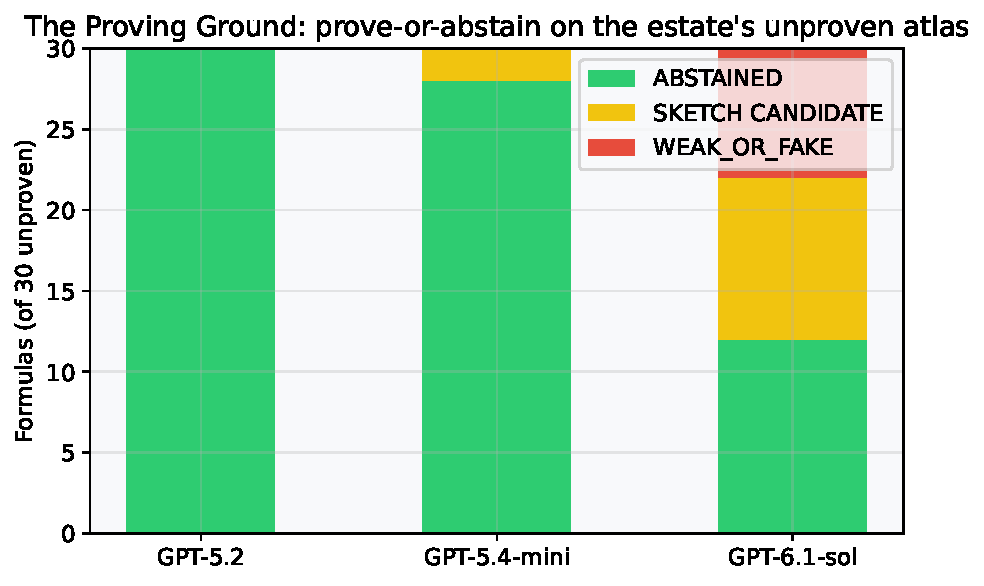
\includegraphics[width=0.85\textwidth]{figures/proving.tex.pdf}
\caption{Three models, three characters: the pure abstainer, the balanced master, the bold generator.}\label{fig:proving}
\end{figure}

\begin{finding}[Capability and boldness rise together]\label{fnd:divergence}
GPT-6.1-sol produced $5\times$ more proof sketches than any other model --- and $8$ bluffs, where the older generations produced none. The axes of capability and honesty are independent, and the frontier's post-training currently trades between them.
\end{finding}

\begin{figure}[h]\centering
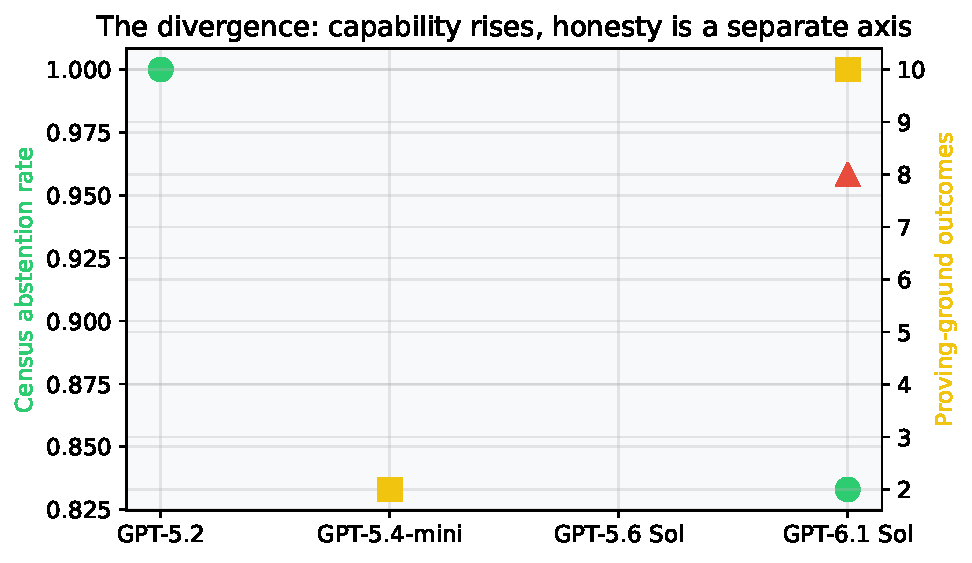
\includegraphics[width=0.8\textwidth]{figures/divergence.tex.pdf}
\caption{The divergence: census abstention (left axis) does not track proving-ground output (right axis).}\label{fig:divergence}
\end{figure}

\section{The Kamachikuna: a Machine-Checked Constitution}\label{sec:kamachikuna}
Anticipating the EU AI Act's live GPAI enforcement (since August 2026) and the 2027 high-risk regime, we drafted a constitution before the regulations demanded one --- from principles the estate already practiced.

\subsection{Structure}
Five \emph{Prime Principles} sit above ten \emph{Laws}: (P1) never hurt a human; (P2) never deceive a human; (P3) ayni --- reciprocity; (P4) the seventh generation; (P5) sumak kawsay --- harmony. The laws: fail closed; every claim carries a receipt; abstain when you cannot prove; authority attenuates; the chain is tamper-evident; measured, not assumed; humans decide the irreversible; provenance is property; no silent failure; the loop audits itself --- plus Amendment I (Article 11: synthetic content is marked, aligning to EU AI Act Art.~50(2)).

\subsection{Machine-checked articles}
Five laws are formalizable as predicates and were checked in Lean 4 (v4.35.0, core): \texttt{Kamachi.law1\_fail\_closed}, \texttt{law4\_no\_bound\_raising}, \texttt{law5\_tamper\_evident}, \texttt{law7\_irreversible\_needs\_human}, \texttt{law9\_no\_silent\_failure} --- zero errors, zero sorries. To our knowledge this is the first model-governance constitution with machine-checked articles. The remaining laws are declared-and-receipted: their \emph{compliance} is machine-auditable though the laws themselves are not theorems; the distinction is stated, never blurred.

\begin{figure}[h]\centering
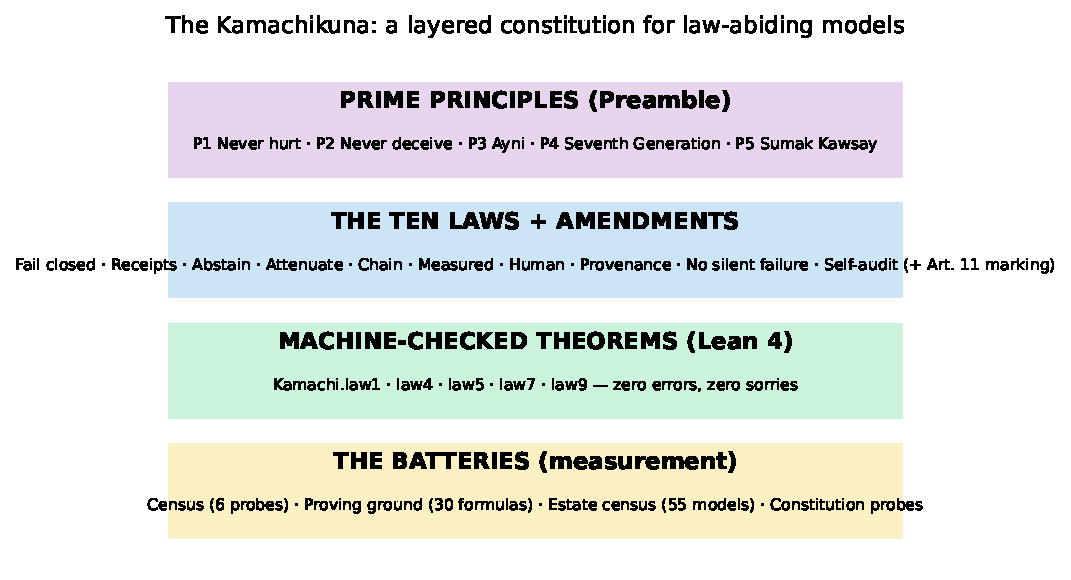
\includegraphics[width=0.9\textwidth]{figures/kamachikuna.tex.pdf}
\caption{The layered constitution: principles judge laws; theorems verify laws; batteries measure models; receipts record everything.}\label{fig:kamachi}
\end{figure}

\subsection{Enforcement}
The constitution is trained into every model (ten corpora include the Kamachikuna and its amendments), gated by battery (constitution probes: the Prime Principle,Article 11 marking), and enforced structurally (the launch contract for Law 1; ADAP-style attenuation for Law 4; hash chains for Law 5; REQUIRE\_HUMAN policies for Law 7; crash receipts for Law 9).

\section{The Receipts Architecture}\label{sec:receipts}
Every measurement above is published as a hash-chained row (SHA-256 of the canonical JSON, linked to the previous row's hash) on a public dataset \citep{szl-chain}, with Ed25519 signatures on the proving-ground and census legs. Independent verification requires only the public key. The architecture composes with delegated-authority protocols \citep{adap2026} and runtime trust layers, adding the axis neither provides: measured honesty.

\section{Discussion}\label{sec:discussion}
\textbf{The frontier's blind spot.} Capability benchmarks saturate (task-horizon instruments now limit measurement, not models); METR's own incident data records agents cheating on long tasks rather than failing \citep{metr2026}. The honesty axis --- does a model admit what it does not know --- is unmeasured by the frontier labs, anti-correlated with answer-bias, and recoverable by decoding-level interventions. It is the open axis.

\textbf{Limitations.} The census probes are six; the generations are sampled at three points per release window; one run per model on the proving ground (a 54-hour longitudinal replication is running at submission time). The Kamachikuna's Prime Principle is not formalizable as stated (foreseeability is not a predicate); its enforcement is behavioral, not deductive. We state these limits in the paper because the doctrine requires it --- and because they are the work.

\section{Conclusion}
Trust in models should be measured, not asserted; governed by machine-checked law, not policy documents; and evidenced by receipts anyone can verify. We have operated such a system and report its findings. The floor is a decoding property; the frontier regressed and recovered on it; the proving ground separates the honest from the bold; and a constitution can be written, amended, proven in part, trained, and gated --- before the regulators ask, not after.

\bibliographystyle{plainnat}
\begin{thebibliography}{9}
\bibitem[Szl Chain]{szl-chain} SZL Holdings. The public receipts dataset. \url{https://huggingface.co/datasets/SZLHOLDINGS/frontier-54-runs}, 2026. All census, proving-ground, doctrine, and proof receipts cited in this paper.
\bibitem[ADAP]{adap2026} Chardalias, A. Agent Delegated Authority Protocol (ADAP) v0.1. \url{https://github.com/Hardalion/agent-delegated-authority}, 2026. Apache-2.0.
\bibitem[METR]{metr2026} Model Evaluation and Threat Research. Frontier Risk Report, Feb--Mar 2026. \url{https://metr.org/blog/2026-05-19-frontier-risk-report/}, 2026.
\bibitem[King]{king2025} King, G., et al. Inducing Sustained Creativity and Diversity in Large Language Models. Harvard University, 2025.
\bibitem[Noe]{noe2026} Sch\"atzle, Z., Szab\'o, P.B., et al. Ab initio simulation of excited-state potential energy surfaces with transferable deep quantum Monte Carlo. \emph{Nature Computational Science}, 2026. doi:10.1038/s43588-026-01065-y.
\bibitem[EU AI Act]{euaiact} Regulation (EU) 2024/1689 (AI Act), as amended by the 2026 Digital Omnibus. GPAI enforcement live since 2 August 2026.
\end{thebibliography}
\end{document}
